\documentclass[11pt]{report}

\usepackage[T1]{fontenc}
\usepackage[polish]{babel}
\usepackage[utf8]{inputenc}
\usepackage{lmodern}
\usepackage[pdftex]{graphicx}
\selectlanguage{polish}
\usepackage[top=3cm, bottom=3cm, left=3cm, right=3cm]{geometry}

\title{Tytuł naszej pracy inżynierskiej}

\begin{document}

%
% przeczytaj: http://en.wikibooks.org/wiki/LaTeX/Document_Structure
%

\maketitle
\tableofcontents

\chapter{Wstęp}

\section{Kontekst zagadnienia}
\par Problem układania planu zajęć dotyczy wielu instytucji głównie związanych ze szkolnictwem, od szkoły podstawowej aż to szkół wyższych. Zadanie sprowadza się do przygotowania graficznego rozkładu zajęć np. dla poszczególnych klas - uczniów uczęszczających do danej klasy, planu zajęć dla każdego z uczących nauczycieli oraz rozkładu zajęć dla każdej sali. Układanie planów zajęć nawet dla niewielkiej szkoły wymaga dużego wysiłku oraz nakładu czasowego. Problem staje jeszcze bardziej skomplikowany dla szkół ponadgimnazjalnych, do których uczęszcza więcej uczniów, tym samym jest więcej klas, nauczycieli oraz realizowanych przedmiotów. Ponadto zagadnienie ułożenia planu zajęć dla szkół wyższych, w których studenci mogą sami wybierać przedmioty w znacznym stopniu komplikuje te zagadnienie. Wynika to z tego, że aby dany plan zajęć był właściwy musi on spełniać podstawowe kryteria: dwa różne zajęcia na które jest zapisany minimum jeden student nie mogą się odbywać w tym samym czasie, dwa różne zajęcia w tym samym czasie nie mogą odbywać się w tej samej sali oraz nauczyciel w danym momencie może nauczać tylko jednego przedmiotu. Rozszerzeń tych ograniczeń jest wiele, a uwzględnienie każdego z nich, często konieczne do stworzenia realnego planu zajęć jest niezbędne. Wprowadzanie kolejnych ograniczeń znacznie utrudnia problem, który i tak jest stosunkowo skomplikowany.
\par Pomysł tematu pracy inżynierskiej wyniknął z przyglądania się na przestrzeni naszej edukacji planom zajęć które często odbiegały od idealnego według naszej opini. Plan zajęć często zawierał sporo przerw między obowiązkowymi zajęciami, zajęcia zaczynały się bardzo wcześnie lub kończyły bardzo późno, co w znacznym stopniu utrudniało powrót do domu bądź też dopasowanie innych poza uczelnianych zajęć do naszego planu.
\par Problem ułożenia planu zajęć podejmowany był w wielu pracach naukowych również na Politechnice Gdańskiej, co świadczy o tym że ułożenie bezkonfliktowego planu zajęć jest problemem stosunkowo trudnym do rozwiązania a zarazem bardzo ciekawym, ponieważ w bezpośredni sposób dotyczy każdej uczącej się osoby. Dlatego też na przestrzeni wielu lat powstało wiele różnych podejść do tego problemu od algorytmów klasycznych poprzez różnego typu algorytmy sztucznej inteligencji.
\par Problem układania graficznych rozkładów nie tylko związany jest ze szkolnictwem, ale również dotyczy konieczności ułożenia rozkładów jazdy komunikacji miejskiej \cite{com}
, planu zajęć dla pracowników \cite{worker} oraz terminarza zawodów sportowych \cite{sport}.
\section{Cel pracy}
\par Celem pracy jest zapoznanie się z problemem układania planów zajęć oraz przegląd różnych sposobów rozwiązania tego problemu. Jak również opracowanie, implementacja oraz porównanie działania wybranych przez nas algorytmów do układania planów zajęć : Algorytm Symulowanego wyżarzania (Particle Swarm Optimization), Algorytm Genetyczny (Genetic Algorithm) oraz Adaptacyjny Algotym Tabu (Adaptive Tabu Search). Stworzone algorytmy mają układać plan zajęć dla wyspecyfikowanego problemu, uwzględniając ograniczenia miękkie oraz ograniczenia twarde. 
\par Dodatkowo podjęliśmy się implementacji systemu w którym użytkownik będzie miał możliwość wygenerowania planu zajęć wybranym przez siebie algorytmem oraz wyświetlenia stworzonego planu zajęć w Google Calendar.
\par W ramach projektu planowane jest również dostosowanie realnych danych ze szkoly ponadgimnazjalnej do zaimplementowanych przez nas algorytmów.
\section{Zakres pracy}
\section{Podział zadań i obowiązków}
\chapter{Opis problemu układania planu zajęć}
\chapter{Specyfikacja problemu}
\section{Sformułowanie problemu}
Celem jest stworzenie tygodniowego harmonogramu wykładów dla kilku kursów, z określoną liczbą dostępnych sal i przedziałów czasowych, w których mogą odbywać się zajęcia. Każdy wykład będący w programie danego kursu musi być przypisany do określonego przedziału czasu i sali tak by spełniał wejściowe ograniczenia. 
\subsection{Jednostki problemu}
\begin{itemize}
\item \textbf{Dni, przedziały, okresy} - dzień podzielony jest na określoną liczbę przedziałów czasowych, okres para złożona z dnia i przedziału czasowego.
\item \textbf{Kursy i wykładowcy} - każdy kurs składa się z określonej liczby wykładów, które muszą być rozłożone w różnym czasie, na które uczęszcza określona liczna studentów i prowadzone są one przez wykładowcę. Dla każdego kursu jest określona minimalna liczba dni w których te wykłady muszą się odbyć, oraz okresy w których dane wykłady nie mogą się odbywać.
\item \textbf{Sale wykładowe} - sale wykładowe mają ograniczoną liczbę dostępnych miejsc w pomieszczeniu.
\item \textbf{Program nauczania} - składa się z kilku kursów, na które uczęszcza grupa studentów.
\end{itemize}
\subsection{Ograniczenia}
\subsubsection{Ograniczenia twarde}
Plan jest wykonywalny - czyli możliwy do realizacji, jeżeli żadne z wymienionych poniżej ograniczeń nie jest naruszone.
\begin{itemize}
\item  ${H_{1}}$ \textbf{Wykłady} - każdy kurs wchodzący w skład programu nauczania musi być przypisany do różnego okresu.
\item  ${H_{2}}$ \textbf{Zajętość sali} - żadne dwa wykłady nie mogą odbywać się w tym samym okresie w jednym pomieszczeniu.
\item  ${H_{3}}$ \textbf{Konflikty pomiędzy kursami} - zajęcia z tego samego programu nauczania bądź nauczanie przez tego samego wykładowcę muszą odbywać się w różnym czasie.
\item  ${H_{4}}$ \textbf{Dostępność wykładowcy} - zajęcia nie mogą się odbywać w czasie, w którym dany wykładowca nie może prowadzić zajęć.
\end{itemize}
\subsubsection{Ograniczenia miękkie}
Ograniczenia te nie wpływają w bezpośredni sposób na wykonalność planu zajęć, ale na jego jakość uwzględniając poniższe kryteria, które wpływają na funkcję oceny wygenerowanego planu zajęć.
\begin{itemize}
\item  ${S_{1}}$ \textbf{Wielkość sali} - liczba studentów uczęszczajacych na zajęcia w danej sali musi być mniejsza bądź równa liczbie dostępnych miejsc.
\item  ${S_{2}}$ \textbf{Stabilność pomieszczenia} - zajęcia wchodzące w skład jednego kursu powinny odbywać się w jednej tej samej sali, jeżeli jest to niemożliwe liczba sal w których odbywają się te zajęcia powinna być jak najmniejsza.
\item  ${S_{3}}$ \textbf{Minimalna liczba dni} - minimalna liczba dni na które powinny być rozłożone zajęcia z danego kursu.
\item  ${S_{4}}$ \textbf{Zwartość zajęć} - zajęcia wchodzące w skład jednego kierunku powinny być w jak najmniejszych odstępach czasu pomiędzy sobą.
\end{itemize}
\subsection{Matematyczne sformułowanie problemu} \cite{tabu}
\par Na problem składa się ${n}$ kursów ${C = \{c_{1}, c_{2},...,c_{n}\}}$ które powinny być przydzielone do ${p}$ różnych okresów ${T = \{t_{1}, t_{2},...,t_{p}\}}$ oraz ${m}$ pomieszczeń w których mogą odbywać się zajęcia ${R = \{r_{1}, r_{2},...,r_{m}\}}$. Okres jest to para składająca się z dnia i przedziału czasowego (${d}$ - liczba dni a ${h}$ - liczba dziennych przedziałów czasowych, czyli ${p = d * h}$). Każdy z kursów składa się z ${n}$ zajęć ${L = \{l_{1},l_{2},...,l_{n}\}}$. Kursy wchodzą w skład ${s}$ programów nauczania ${CR = \{cr_{1}, cr_{2}, ..., cr_{s}\}}$, na program nauczania składają się kursy, na które uczęszczają ci sami studenci. 
\par Problem definiujemy w postaci macierzy ${X}$  rozmiaru ${p * m}$ gdzie ${x_{i,j}}$ który definiuje przypisanie danych zajęć do ${t_{j}}$ okresu oraz sali ${r_{i}}$. Jeżeli w danym czasie w danej sali nie odbywają się zajęcia wartość ${x_{i,j}}$ będzie przyjmowała wartość ${null}$. Dzięki takiemu sposobowi zdefiniowania problemu nigdy nie zostanie naruszone ograniczenie twarde ${H_{2}}$ dotyczące zajętości sali.
\chapter{Opis zrealizowanych algorytmów}
\section{Adaptive tabu search}
\subsection{Ogólny opis algorytmu}
\par Opis zaimplementowanego przez nas algorytmu został zaczerpnięty z pracy ,,Adaptive TabuSearch for Course Timetabling'' \cite{tabu}
\par Na całość algorytmu składają się trzy fazy: faza inicjalizacji podczas której tworzony jest początkowy plan zajęć, przy pomocy zachłannej heurystyki, faza intensyfikacji, która jest właściwą fazą algorytmu Tabu Search, której celem jest optymalizacja funkcji oceny ograniczeń miękkich. Końcowa faza - faza dywersyfikacji gdzie dokonywana jest redukcja naruszeń miękkich, tak aby nie łamać twardych ograniczeń. Na algorytm ten składa się wiele unikalnych cech między innymi struktury sąsiedztwa - podwójne łańcuchy Kempe, operator zaburzeń oraz dynamiczna integracja operacji przeszukiwania tabu z operatorem zaburzeń.
\subsection{Fazy algorytmu}
\subsubsection{Faza inicjalizacji}
\subsubsection{Faza intensyfikacji}
\subsubsection{Faza dywersyfikacji}
\section{Particle Swarm Optimization}
\section{Genetic Algorithm}
\subsection{Ogólny opis algorytmu}
\par Algorytm genetyczny to rodzaj algorytmu przeszukującego przestrzeń alternatywnych rozwiązań problemu w celu wyszukania rozwiązań najlepszych. Obecnie zalicza się go do grupy algorytmów ewolucyjnych.
\par Algorytmy genetyczne zajmują bardzo ważne miejsce w dziedzinie projektowania i analizy algorytmów. Doskonale sprawdzają się w sytuacji, gdy problem, z którym przychodzi nam się zmierzyć, jest nie do rozwiązania w sposób klasyczny w sensownym czasie. Pozwalają znaleźć sub-optymalne rozwiązanie problemów, których dziedziny nie są łatwe do wyznaczenia. Są powszechnie stosowane tam, gdzie do uzyskania rozwiązania korzystamy z zagadnień sztucznej inteligencji oraz tam, gdzie uzyskanie rozwiązania jest bardzo złożonym problem, natomiast jego ocena jest łatwa i błyskawiczna.
\par Należy zaznaczyć, że algorytm genetyczny nie gwarantuje znalezienia rozwiązania optymalnego, lecz przybliżone. Istota jego działania jest zbliżona do charakterystycznych dla środowiska naturalnego procesów ewolucyjnych. Cały algorytm operuje na grupie (populacji) potencjalnych rozwiązań, których jakość (stopień, w jakim jest bliskie rozwiązania optymalnego) potrafimy ocenić i które zbliżają się w przypominającym ewolucyjny procesie do rozwiązania optymalnego.
\par Problem definiuje środowisko, w którym istnieje pewna populacja osobników. Każdy z osobników ma przypisany pewien zbiór informacji stanowiących jego genotyp, a będących podstawą do utworzenia fenotypu. Fenotyp to zbiór cech podlegających ocenie funkcji przystosowania modelującej środowisko. Innymi słowy - genotyp opisuje proponowane rozwiązanie problemu, a funkcja przystosowania ocenia, jak dobre jest to rozwiązanie. Genotyp składa się z chromosomów, gdzie zakodowany jest fenotyp i ewentualnie pewne informacje pomocnicze dla algorytmu genetycznego. Chromosom składa się z genów.
\par Najczęściej działanie algorytmu przebiega następująco:
\begin{enumerate}
\item Losowana jest pewna populacja początkowa.
\item Populacja poddawana jest ocenie (selekcja). Najlepiej przystosowane osobniki biorą udział w procesie reprodukcji.
\item Genotypy wybranych osobników są ze sobą kojarzone poprzez złączanie genotypów rodziców (krzyżowanie).
\item Przeprowadzana jest mutacja, czyli wprowadzenie drobnych losowych zmian.
\item Rodzi się kolejne pokolenie. Aby utrzymać stałą liczbę osobników w populacji te najlepsze (według funkcji oceniającej fenotyp) są powielane, a najsłabsze usuwane. Jeżeli nie znaleziono dostatecznie dobrego rozwiązania, algorytm powraca do kroku drugiego. W przeciwnym wypadku wybieramy najlepszego osobnika z populacji - jego genotyp to uzyskany wynik.
\end{enumerate}
\subsection{Historia i zastosowanie}
Sposób działania algorytmów genetycznych nieprzypadkowo przypomina zjawisko ewolucji biologicznej, ponieważ ich twórca John Henry Holland właśnie z biologii czerpał inspiracje do swoich prac. 
\subsection{Fazy algorytmu}
\subsubsection{Utworzenie rozwiązania początkowego}
\subsubsection{Selekcja}
\subsubsection{Krzyżowanie}
\subsubsection{Mutacja}
\subsubsection{Elityzm}
\subsection{Istniejące implementacje}
\chapter{Projekt systemu}
\subsection{Zastosowanie}
\subsubsection{Przypadki użycia}
\par
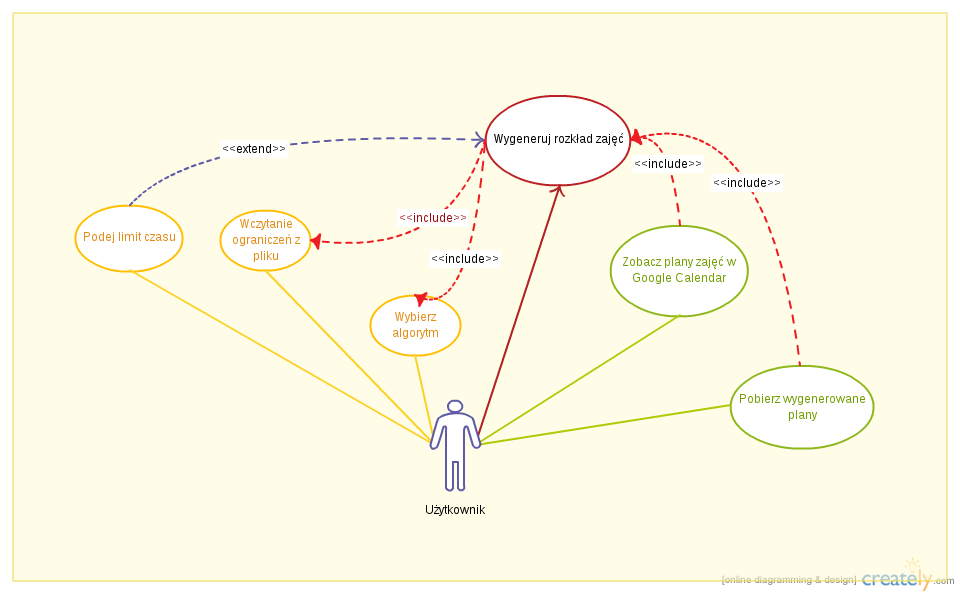
\includegraphics[width=0.8\textwidth]{InzynierkaUseCase.png}
\subsection{Architektura systemu}
\par
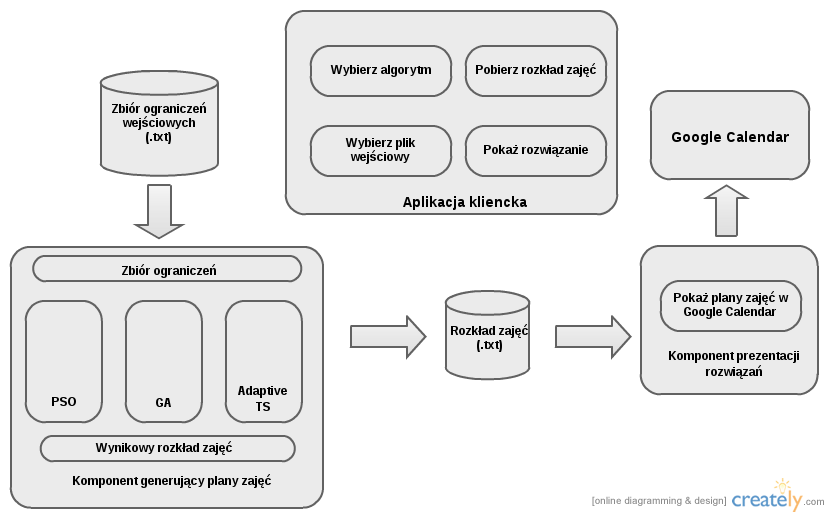
\includegraphics[width=0.8\textwidth]{ComponentsDiagram.png}
\chapter{Testy}
\chapter{Porównanie algorytmów}
\chapter{Sposób użytkowania systemu}
\chapter{Podsumowanie}

\begin{thebibliography}{2}
\bibitem{tabu} Zhipeng Lu, Jin-Kao Hao. Adaptive TabuSearch for Course Timetabling.  \emph{European Journal of Operational Research}, 200(1):235-244, 2010.
\bibitem{com} U. Brannlund, P. ). Lindberg, A. Nou, J. E. Nilsson. Timetabling using lagrangian relaxation Transportation Science 32, 358-369, 1998
\bibitem{sport} J. A. M. Schreuder. Constructing timetables for sport competitions. \emph{Mathematical Programming Study 13}, 58-67, 1980
\bibitem{worker} M. Chiarandini, A. Schaerf, F. Tiozzo. Solving employee timetabling problems with flexible workload using tabu search. \emph{Proceedings of the 3rd PATAT Conference}, 2013
\end{thebibliography}

\end{document}
